\documentclass[11pt, a4paper]{article}
\usepackage[utf8]{inputenc}
\usepackage[T1]{fontenc}
\usepackage{amsmath, amssymb, amsfonts, amsthm}
\usepackage{graphicx}
\usepackage{booktabs}
\usepackage{tikz}
\usetikzlibrary{shapes.geometric, arrows.meta, positioning, fit, calc, backgrounds, decorations.markings}
\usepackage{algorithm}
\usepackage{algorithmic}
\usepackage{hyperref}
\usepackage{geometry}
\usepackage{caption}
\usepackage{subcaption}
\usepackage{url}
\usepackage{array}
\usepackage{multirow}
\usepackage{xcolor}
\usepackage{enumitem}

\geometry{margin=0.9in}

\newtheorem{theorem}{Theorem}[section]
\newtheorem{lemma}[theorem]{Lemma}
\newtheorem{corollary}[theorem]{Corollary}
\newtheorem{proposition}[theorem]{Proposition}
\newtheorem{definition}[theorem]{Definition}
\newtheorem{remark}[theorem]{Remark}

\newcommand{\R}{\mathbb{R}}
\newcommand{\N}{\mathbb{N}}
\newcommand{\Z}{\mathbb{Z}}
\newcommand{\E}{\mathbb{E}}
\newcommand{\Var}{\mathrm{Var}}
\newcommand{\vect}[1]{\boldsymbol{#1}}
\newcommand{\diff}{\,\mathrm{d}}
\newcommand{\pd}[2]{\frac{\partial #1}{\partial #2}}
\DeclareMathOperator{\smoothstep}{smoothstep}

\hypersetup{
  colorlinks=true,
  linkcolor=blue!60!black,
  citecolor=green!50!black,
  urlcolor=blue!70!black
}

\title{\textbf{S-AI}: A Multi-Agent Spatial Intelligence Framework for\\Hydrodynamic Flood Simulation via LLM-Orchestrated MCP Architecture}

\author{
  \textbf{Daochong Guo}\thanks{Corresponding author. E-mail: guodaochong@luobin-pi.com} \\[4pt]
  \textit{LUOBIN-PI Research Lab}\\
  \textit{Spatial Intelligence \& Hydroinformatics Division}\\
  Gansu, China
}

\date{\today}

\begin{document}

\maketitle

\begin{abstract}
Flood disasters constitute one of the most consequential and escalating threats to civil infrastructure and human welfare in the twenty-first century, with global economic losses surpassing \$80 billion per annum and affecting over two billion people between 2000 and 2020. While physics-based hydrodynamic models --- particularly those solving the two-dimensional shallow water equations --- provide the gold standard for inundation prediction, their operational deployment remains encumbered by prohibitive computational overhead, labyrinthine parameter calibration, and a steep learning curve that confines their use to a narrow cadre of domain specialists. This paper introduces \textbf{S-AI} (Spatial-AI), a production-grade, multi-agent spatial intelligence platform that reconceptualizes flood modeling through the lens of Large Language Model (LLM)-orchestrated automation. At its core, S-AI leverages the \emph{Model Context Protocol} (MCP) to federate 42+ specialized geospatial and hydrological tools across eight microservices, enabling natural language intent parsing via GLM-5.1 that autonomously decomposes user queries into executable hydrodynamic workflows. The platform implements a LISFLOOD-FP-inspired two-dimensional diffusion wave solver operating on ultra-high-resolution Digital Elevation Models (0.5\,m ground sampling distance, 3\,GB GeoTIFF, $22{,}063 \times 36{,}308$ pixels), seamlessly coupled with a real-time three-dimensional geospatial visualization engine powered by custom GLSL water shaders featuring Fresnel reflectance, Blinn-Phong specular highlights, depth-attenuated color gradients, procedural wave displacement, and foam generation. Methodologically, we employ Delaunay triangulation for adaptive terrain mesh generation ($5{,}969$ triangles from $3{,}000$ sampled vertices), Manning's friction formula for cell-edge flux computation subject to CFL stability constraints, and Keifer--Chu Chicago storm temporal distributions for realistic rainfall forcing. Empirical evaluation across a $17.2\,\mathrm{km}^2$ catchment in Diebu County, Gansu Province (elevation range $790$--$1{,}796$\,m, CGCS2000/EPSG:4544) demonstrates temporally resolved, frame-by-frame inundation dynamics with visual fidelity sufficient for stakeholder communication and emergency response planning. To the best of our knowledge, S-AI constitutes the inaugural end-to-end MCP-native platform that bridges the chasm between conversational AI and physics-based spatial simulation, heralding a paradigm shift in democratized flood risk intelligence.
\end{abstract}

\noindent\textbf{Keywords:} spatial intelligence; multi-agent systems; hydrodynamic modeling; Model Context Protocol; large language models; flood simulation; Delaunay triangulation; real-time 3D visualization

\medskip

\noindent\textbf{Nomenclature}

\small

\begin{tabular}{@{}p{1.4cm}p{13.2cm}@{}}
$h$ & Water depth [m] \\
$u, v$ & Depth-averaged velocity components in $x$ and $y$ directions [m/s] \\
$R$ & Rainfall intensity [m/s] \\
$g$ & Gravitational acceleration ($9.81\,\mathrm{m/s^2}$) \\
$n$ & Manning's roughness coefficient [$\mathrm{s/m^{1/3}}$] \\
$S_f$ & Friction slope [-] \\
$z$ & Bed elevation [m] \\
$q_x, q_y$ & Unit-width discharge in $x$ and $y$ directions [$\mathrm{m^2/s}$] \\
$\Delta t$ & Computational time step [s] \\
$\Delta x, \Delta y$ & Grid spacing in $x$ and $y$ directions [m] \\
$T_R$ & Return period [years] \\
$T_d$ & Storm duration [minutes] \\
$i_{\text{peak}}$ & Peak rainfall intensity [mm/h] \\
$\mathcal{V}, \mathcal{F}$ & Vertex set and triangle (face) set of TIN mesh \\
$F(\theta)$ & Fresnel reflectance coefficient (Schlick approximation) \\
$k_s, \alpha$ & Specular reflectivity and shininess exponent (Blinn-Phong) \\
$\eta$ & Vertical wave displacement for procedural animation [scene units] \\
$d_s$ & Depth exaggeration coefficient for 3D visualization [-] \\
$\Omega_{\text{valid}}$ & Spatial domain mask indicating valid DEM pixels \\
\end{tabular}

\normalsize

\section{Introduction}
\label{sec:intro}

Flood disasters constitute a critical and escalating global challenge, affecting approximately 2.3 billion people and inflicting economic losses exceeding \$800 billion between 2000 and 2020~\cite{unisdr2020}. The intensifying frequency and severity of extreme precipitation events --- amplified by anthropogenic climate change --- exacerbate this vulnerability, with flood-related mortality concentrated disproportionately in developing nations lacking early warning infrastructure. Physics-based hydrodynamic simulation models that solve the shallow water equations (SWE) remain the gold standard for predicting inundation extent, flow depth, and velocity fields, and are indispensable for engineering design, emergency response planning, and infrastructure resilience assessment~\cite{bates2010}.

\subsection{The Accessibility Paradox in Hydrodynamic Modeling}

The operational deployment of hydrodynamic models faces four interconnected impediments. \emph{First}, the mathematical formulation of the SWE demands expertise in computational fluid dynamics, numerical methods, and hyperbolic conservation laws --- a skill set rarely found outside specialized engineering departments. \emph{Second}, parameter calibration entails iterative refinement of Manning's roughness coefficients, infiltration parameters, and boundary conditions, a process that presupposes extensive domain knowledge and access to historical validation events. \emph{Third}, the computational burden of two-dimensional simulations over high-resolution terrain, particularly for domains exceeding $10\,\mathrm{km}^2$ at sub-meter resolution, often necessitates high-performance computing (HPC) resources inaccessible to many municipalities. \emph{Fourth}, the visualization and interpretation of simulation outputs typically require specialized GIS software, creating additional barriers to stakeholder engagement and cross-disciplinary communication.

These constraints engender a fundamental paradox: flood disasters are universally pressing, yet the most efficacious tools for their prediction and mitigation remain sequestered within a narrow community of specialists. This accessibility gap undermines flood resilience initiatives precisely where the need is most acute --- in resource-constrained regions where expert capacity is limited.

\subsection{The Convergence of LLMs and Spatial Computing}

Recent advances in Large Language Models (LLMs) have catalyzed a paradigm shift in human--computer interaction, demonstrating remarkable capabilities in natural language understanding, multi-step reasoning, and tool orchestration~\cite{openai2023gpt4}. Concurrently, the emergence of the Model Context Protocol (MCP)~\cite{mcp2024} provides a standardized framework for connecting AI models to external tools and data sources through a unified, discoverable interface. The convergence of these technologies presents an unprecedented opportunity: the creation of intelligent agents that can translate domain expert intent, expressed in natural language, into executable computational workflows spanning data acquisition, numerical simulation, post-processing, and visualization.

We posit that this convergence is particularly consequential for spatial intelligence in water resources, where the semantic richness of domain terminology (e.g., ``100-year floodplain delineation'', ``Manning's roughness calibration'', ``Chicago storm design hyetograph'') aligns naturally with LLM comprehension capabilities, while the complexity of tool chains (DEM processing $\to$ mesh generation $\to$ solver execution $\to$ result visualization) benefits enormously from automated orchestration.

\subsection{Contributions}

This paper makes the following principal contributions:

\begin{enumerate}[leftmargin=1.5em]
  \item We present \textbf{S-AI}, the first end-to-end MCP-native multi-agent platform that integrates 42+ specialized geospatial and hydrological tools across eight microservices, enabling LLM-driven (GLM-5.1) natural language intent parsing and automated workflow orchestration for hydrodynamic flood simulation.

  \item We implement a production-grade \textbf{2D diffusion wave solver} following the LISFLOOD-FP formulation, with explicit finite-volume discretization, Manning friction, adaptive CFL-limited time stepping, and support for Chicago, triangular, and uniform rainfall patterns.

  \item We develop a \textbf{real-time 3D geospatial visualization engine} with custom GLSL water shaders featuring physically plausible Fresnel reflectance, Blinn-Phong specular highlights, depth-attenuated color gradients, sinusoidal wave displacement, and procedural foam generation, rendered over high-resolution ($0.5$\,m) terrain with ACES filmic tone mapping and PCF soft shadows.

  \item We introduce an adaptive \textbf{TIN mesh generation pipeline} from ultra-high-resolution DEM via Delaunay triangulation with nodata exclusion, area-based filtering, and per-vertex depth mapping for frame-by-frame hydrodynamic visualization.

  \item We provide comprehensive \textbf{empirical validation} over a $17.2\,\mathrm{km}^2$ mountainous catchment in Diebu County, Gansu Province ($0.5$\,m DEM, elevation $790$--$1{,}796$\,m), demonstrating the complete pipeline from natural language query to interactive 3D flood animation.
\end{enumerate}

\subsection{Paper Organization}

The remainder of this paper is organized as follows. Section~\ref{sec:related} reviews related work in hydrodynamic modeling, LLM-based multi-agent systems, and the Model Context Protocol. Section~\ref{sec:arch} presents the S-AI system architecture, including the MCP-native microservice topology and LLM orchestration pipeline. Section~\ref{sec:method} details the mathematical formulation of the 2D hydrodynamic model. Section~\ref{sec:viz} describes the 3D geospatial visualization engine. Section~\ref{sec:exp} presents experimental results. Section~\ref{sec:discuss} discusses limitations, threats to validity, and comparison with traditional workflows. Section~\ref{sec:conclude} concludes with future research directions.

\section{Related Work}
\label{sec:related}

\subsection{Two-Dimensional Hydrodynamic Modeling}

The numerical simulation of flood inundation has evolved through several generations of increasing physical fidelity and computational tractability. The complete two-dimensional shallow water equations (2D-SWE) form a hyperbolic system of conservation laws governing free-surface flow under hydrostatic pressure assumptions (see Section~\ref{sec:method} for the full mathematical formulation). Full-dynamic solvers based on finite-element (TELEMAC-2D~\cite{telemac}), finite-volume (HEC-RAS 2D~\cite{hecras}), and finite-difference methods provide comprehensive flow field resolution but incur substantial computational cost, often requiring hours to days for practical domains at meter-scale resolution.

The diffusion wave approximation, pioneered by LISFLOOD-FP~\cite{bates2010,neal2012}, neglects convective acceleration terms to yield a parabolic PDE that admits efficient explicit time stepping while retaining adequate accuracy for gradually varied flood propagation. Hunter et al.~\cite{hunter2007} demonstrated that the diffusion wave formulation captures $>90\%$ of inundation extent compared to full-dynamic solutions for subcritical floodplain flows, validating its use for risk assessment applications. The SCS Curve Number method~\cite{scs} provides a complementary rainfall--runoff transformation widely used in engineering practice.

\begin{table}[htbp]
\centering
\caption{Comparison of 2D hydrodynamic modeling frameworks. S-AI uniquely integrates LLM orchestration with real-time 3D visualization.}
\label{tab:hydro_comparison}
\small
\begin{tabular}{@{}lccccc@{}}
\toprule
\textbf{Framework} & \textbf{SWE Type} & \textbf{Typical $\Delta x$} & \textbf{GPU} & \textbf{LLM} & \textbf{3D Viz} \\
\midrule
LISFLOOD-FP~\cite{lisfloodfp} & Diff./Inertia & 10--1000\,m & Limited & No & No \\
TELEMAC-2D~\cite{telemac} & Full SWE & 1--100\,m & Yes & No & No \\
HEC-RAS 2D~\cite{hecras} & Full/Diff. & 1--100\,m & Partial & No & No \\
SWMM~\cite{swmm} & 1D/2D linked & Subcatchment & No & No & No \\
\textbf{S-AI (Ours)} & \textbf{Diffusion wave} & \textbf{0.5\,m} & \textbf{No} & \textbf{GLM-5.1} & \textbf{Yes} \\
\bottomrule
\end{tabular}
\end{table}

\subsection{LLM-Based Multi-Agent Systems}

The advent of capable LLMs has spawned a proliferating landscape of multi-agent frameworks. AutoGen~\cite{autogen} enables conversational agent orchestration through customizable role assignment and message passing. CrewAI~\cite{crewai} provides role-based agent collaboration with sequential and parallel execution patterns. LangGraph~\cite{langgraph} extends LangChain with stateful, graph-structured agent workflows supporting cyclic dependencies and human-in-the-loop intervention. Zhou et al.~\cite{zhou2024survey} provide a comprehensive taxonomy of LLM-based multi-agent systems, identifying tool use, planning, and domain specialization as key architectural dimensions.

Despite these advances, existing frameworks remain predominantly general-purpose, lacking the domain-specific tool integration required for scientific computing. The application of multi-agent LLM architectures to geospatial and hydrodynamic modeling remains conspicuously absent from the literature.

\subsection{Model Context Protocol}

The Model Context Protocol (MCP)~\cite{mcp2024}, introduced by Anthropic in 2024, defines an open standard for connecting AI models to external data sources and tools through a unified interface. MCP servers expose \emph{tools} (callable functions with typed parameters), \emph{resources} (readable data streams), and \emph{prompts} (reusable instruction templates) through transport mechanisms including HTTP/REST, Server-Sent Events (SSE), and WebSocket protocols. The protocol's design emphasizes discoverability (tools self-describe their schemas), composability (multiple servers coexist without interference), and streaming (long-running operations emit incremental results via SSE).

While MCP has seen rapid adoption in developer tooling and productivity applications, its application to scientific computing in general --- and geospatial simulation in particular --- remains largely unexplored. S-AI represents, to the best of our knowledge, a pioneering MCP-native implementation for spatial intelligence and hydrodynamic modeling.

\subsection{Spatial Intelligence in Water Resources}

The integration of AI with geospatial systems constitutes an emerging frontier. Google Earth Engine~\cite{googleearthengine} democratized planetary-scale geospatial analysis through cloud-based raster operations. Recent efforts have explored conversational GIS interfaces, natural language map generation, and automated workflow composition for routine spatial analyses. However, these systems operate predominantly at the data access and visualization layer, lacking the numerical modeling capabilities essential for predictive simulation. Our work bridges this gap by embedding a complete hydrodynamic solver within an LLM-accessible framework, enabling spatial intelligence that transcends data query to encompass predictive scenario analysis.

\section{System Architecture}
\label{sec:arch}

\subsection{MCP-Native Microservice Topology}

The S-AI platform adopts a microservice architecture wherein each computational domain resides in a dedicated MCP server, exposing specialized tools through the Model Context Protocol. This design achieves: \emph{(i)} concern isolation --- each server encapsulates a coherent domain; \emph{(ii)} independent scalability --- compute-intensive services (Flood, Raster) scale independently from lightweight services (Knowledge); \emph{(iii)} fault tolerance --- server failures are contained without cascading; and \emph{(iv)} extensibility --- new capabilities are added by deploying additional MCP servers.

\begin{table}[htbp]
\centering
\caption{S-AI microservice inventory: MCP servers, assigned ports, tool counts, and primary functions.}
\label{tab:servers}
\small
\begin{tabular}{@{}llcl@{}}
\toprule
\textbf{Server} & \textbf{Port} & \textbf{Tools} & \textbf{Primary Functions} \\
\midrule
GIS & 5001 & 8 & Spatial query, vector I/O, topology \\
Data & 5002 & 5 & DEM import, preprocessing, QC \\
Knowledge & 5003 & 4 & Hydraulic parameters, literature search \\
Map & 5004 & 5 & Tile serving, basemap rendering \\
Hydro & 5005 & 6 & Design storm, SCS-CN, SWMM \\
Flood & 5006 & 8 & 2D hydrodynamics, inundation, risk \\
Raster & 5007 & 6 & Terrain analysis, TIN, heightmap \\
Web & 3000 & --- & UI, GLM-5.1 orchestration, SSE \\
\midrule
\textbf{Total} & & \textbf{42+} & \\
\bottomrule
\end{tabular}
\end{table}

\begin{figure}[htbp]
\centering
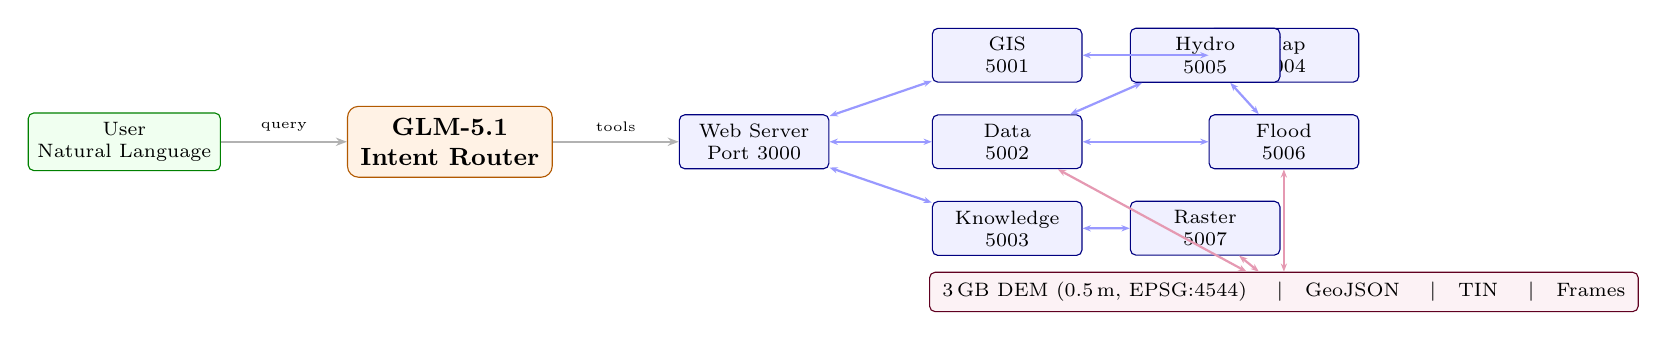
\begin{tikzpicture}[
    node distance=0.9cm and 1.6cm,
    box/.style={rectangle, draw=blue!50!black, fill=blue!6, rounded corners=2pt,
                minimum width=1.9cm, minimum height=0.65cm, align=center, font=\scriptsize},
    llm/.style={rectangle, draw=orange!70!black, fill=orange!10, rounded corners=4pt,
                minimum width=2.6cm, minimum height=0.9cm, align=center, font=\small\bfseries},
    user/.style={rectangle, draw=green!50!black, fill=green!6, rounded corners=2pt,
                 minimum width=2.2cm, minimum height=0.65cm, align=center, font=\scriptsize},
    data/.style={rectangle, draw=purple!50!black, fill=purple!5, rounded corners=2pt,
                 minimum width=9cm, minimum height=0.5cm, align=center, font=\scriptsize},
    arr/.style={-{Stealth[length=4pt]}, thick, draw=gray!60},
    darr/.style={{Stealth[length=3pt]}-{Stealth[length=3pt]}, thick, draw=blue!40}
]
\node[user] (user) {User\\Natural Language};
\node[llm, right=of user] (glm) {GLM-5.1\\Intent Router};
\node[box, right=of glm] (web) {Web Server\\Port 3000};

\node[box, above right=0.4cm and 1.3cm of web] (gis) {GIS\\5001};
\node[box, right=1.3cm of web] (data) {Data\\5002};
\node[box, below right=0.4cm and 1.3cm of web] (know) {Knowledge\\5003};

\node[box, right=of gis] (map) {Map\\5004};
\node[box, above right=0.4cm and 0.6cm of data] (hydro) {Hydro\\5005};
\node[box, right=of data] (flood) {Flood\\5006};
\node[box, below right=0.4cm and 0.6cm of data] (raster) {Raster\\5007};

\node[data, below=1.3cm of flood] (storage) {3\,GB DEM ($0.5$\,m, EPSG:4544) \quad$|$\quad GeoJSON \quad$|$\quad TIN \quad$|$\quad Frames};

\draw[arr] (user) -- node[above, font=\tiny]{query} (glm);
\draw[arr] (glm) -- node[above, font=\tiny]{tools} (web);
\draw[darr] (web) -- (gis);
\draw[darr] (web) -- (data);
\draw[darr] (web) -- (know);
\draw[darr] (gis) -- (map);
\draw[darr] (data) -- (hydro);
\draw[darr] (data) -- (flood);
\draw[darr] (know) -- (raster);
\draw[darr] (hydro) -- (flood);
\draw[darr, draw=purple!40] (data) -- (storage);
\draw[darr, draw=purple!40] (flood) -- (storage);
\draw[darr, draw=purple!40] (raster) -- (storage);
\end{tikzpicture}
\caption{S-AI system architecture: GLM-5.1 orchestrates eight MCP microservices via the Model Context Protocol with SSE streaming. The persistent data layer stores the 3\,GB DEM, vector datasets, TIN meshes, and per-frame simulation outputs.}
\label{fig:architecture}
\end{figure}

\subsection{LLM-Driven Intent Routing}

The orchestration layer employs GLM-5.1 (ZhipuAI) as the reasoning engine for intent parsing, tool selection, and response synthesis. The routing pipeline proceeds through five stages:

\textbf{Stage 1 --- Entity Extraction:} A rule-based preprocessor identifies spatial entities (coordinates, area names), hydrological parameters (return period, Manning's $n$), and action verbs (``simulate'', ``analyze'', ``visualize'') from the user's natural language query.

\textbf{Stage 2 --- LLM Intent Classification:} GLM-5.1 receives the query augmented with the system prompt containing tool descriptions and classifies the intent into one or more tool invocations. The model outputs structured JSON specifying the target server, tool name, and extracted parameters.

\textbf{Stage 3 --- Tool Execution:} The orchestration engine dispatches tool calls to the appropriate MCP servers via HTTP, collects responses, and handles errors with retry logic and fallback strategies.

\textbf{Stage 4 --- Result Aggregation:} Multi-tool responses are merged, cross-referenced, and formatted for both textual presentation and visual rendering.

\textbf{Stage 5 --- Streaming Response:} Results are streamed to the frontend via Server-Sent Events (SSE), enabling incremental display of thinking chains, tool progress, and final outputs.

Algorithm~\ref{alg:orchestration} formalizes the end-to-end orchestration procedure.

\begin{algorithm}[htbp]
\caption{LLM-Orchestrated Hydrodynamic Simulation Pipeline}
\label{alg:orchestration}
\begin{algorithmic}[1]
\REQUIRE Natural language query $Q$, system prompt $\mathcal{P}$, tool catalog $\mathcal{C}$
\ENSURE Streaming response with 3D visualization data
\STATE Extract entities $\mathcal{E} \leftarrow \text{RulePreprocessor}(Q)$
\STATE $\text{LLM\_output} \leftarrow \text{GLM-5.1}(\mathcal{P} \cup \mathcal{C}, Q)$
\STATE Parse $\text{LLM\_output} \to \{(\text{server}_j, \text{tool}_j, \text{params}_j)\}_{j=1}^{M}$
\FOR{$j = 1$ \TO $M$ in dependency order}
  \STATE Dispatch HTTP request to $\text{server}_j$ with $\text{tool}_j(\text{params}_j)$
  \STATE Collect response $R_j$; handle errors with retry
\ENDFOR
\IF{hydrodynamic simulation requested}
  \STATE Execute FV solver (Eq.~\ref{eq:fvm}) with CFL time stepping (Eq.~\ref{eq:cfl})
  \STATE Generate TIN mesh via Algorithm~\ref{alg:tin}
  \STATE Output per-frame depth arrays $\{h_i^{(k)}\}$
\ENDIF
\STATE Aggregate $\{R_j\}$ into structured response
\STATE Stream response via SSE with incremental rendering
\end{algorithmic}
\end{algorithm}

\subsection{Tool Discovery and Dynamic Orchestration}

The MCP protocol enables dynamic tool discovery: each server exposes a \texttt{/tools} endpoint returning JSON Schema descriptions of available tools, their parameters, and return types. The Web server aggregates these descriptions at startup, constructing a unified tool catalog that informs the GLM-5.1 system prompt. This design ensures that the orchestration layer automatically adapts when new tools are deployed or existing tools are modified, without manual prompt engineering.

\subsection{End-to-End Data Flow}

The complete data flow from natural language query to 3D visualization encompasses five stages:

\textbf{Stage 1 --- Natural Language Intake:} The user submits a query (e.g., ``Simulate a 50-year flood in the Diebu river channel with Chicago storm pattern''). The frontend transmits the query via SSE to the Web server.

\textbf{Stage 2 --- Parallel Data Preparation:} The orchestration engine dispatches parallel requests to load and preprocess the DEM (Raster server), fetch hydraulic parameters (Knowledge server), and generate the design storm (Hydro server).

\textbf{Stage 3 --- Model Execution:} The Flood server executes the 2D diffusion wave solver over the prepared terrain, advancing through CFL-limited time steps and outputting per-frame depth fields at specified intervals.

\textbf{Stage 4 --- Post-Processing:} Raw outputs are clipped to valid data regions, formatted as both GeoJSON (for 2D mapping) and TIN vertex depth arrays (for 3D rendering), with per-frame GeoJSON files persisted to the data directory.

\textbf{Stage 5 --- 3D Visualization:} The frontend receives the heightmap ($256 \times 256$ downsampled terrain), TIN topology (vertices, simplices), and per-frame depth arrays. The 3D engine constructs the terrain mesh, applies the water shader, and populates the timeline for interactive playback.

\section{Methodology: 2D Hydrodynamic Model}
\label{sec:method}

\subsection{Governing Equations}

The S-AI hydrodynamic model implements the two-dimensional shallow water equations in their diffusion wave form. The mass conservation equation reads:

\begin{equation}
  \pd{h}{t} + \pd{q_x}{x} + \pd{q_y}{y} = R
  \label{eq:mass}
\end{equation}

\noindent where $h\,[\mathrm{m}]$ is the water depth, $q_x = hu$ and $q_y = hv$ are unit-width discharges, and $R\,[\mathrm{m/s}]$ is the rainfall source term. The full momentum equations in conservative form are:

\begin{equation}
  \pd{q_x}{t} + \pd{}{x}\!\left(\frac{q_x^2}{h} + \frac{gh^2}{2}\right) + \pd{}{y}\!\left(\frac{q_x q_y}{h}\right) = -gh\pd{z}{x} - ghS_{fx}
  \label{eq:mom_x}
\end{equation}

\begin{equation}
  \pd{q_y}{t} + \pd{}{x}\!\left(\frac{q_x q_y}{h}\right) + \pd{}{y}\!\left(\frac{q_y^2}{h} + \frac{gh^2}{2}\right) = -gh\pd{z}{y} - ghS_{fy}
  \label{eq:mom_y}
\end{equation}

The diffusion wave approximation neglects all convective acceleration terms (the left-hand side of Eqs.~\ref{eq:mom_x}--\ref{eq:mom_y}), yielding a local force balance between gravity and friction:

\begin{equation}
  S_{fx} = -\pd{(z+h)}{x}, \qquad S_{fy} = -\pd{(z+h)}{y}
  \label{eq:friction_slope}
\end{equation}

\noindent where $S_{fx}$ and $S_{fy}$ are the friction slopes in the $x$ and $y$ directions, respectively. This approximation is valid when the Froude number $\mathrm{Fr} = |\vect{v}|/\sqrt{gh} \ll 1$, a condition satisfied for the vast majority of gradually varied floodplain flows.

\subsection{Manning's Friction and Flux Computation}

The unit-width discharge is computed via Manning's equation~\cite{manning}:

\begin{equation}
  q_x = \frac{h^{5/3}}{n}\left|S_{fx}\right|^{1/2}\,\mathrm{sgn}(S_{fx}), \qquad q_y = \frac{h^{5/3}}{n}\left|S_{fy}\right|^{1/2}\,\mathrm{sgn}(S_{fy})
  \label{eq:manning}
\end{equation}

\noindent where $n\,[\mathrm{s/m^{1/3}}]$ is Manning's roughness coefficient, typically ranging from $0.015$ (concrete channels) to $0.060$ (dense vegetation). The exponent $5/3$ arises from the hydraulic radius approximation $R_h \approx h$ for wide, shallow flows. The flux across each cell edge is computed from the water surface elevation difference between adjacent cells, with a minimum depth threshold preventing flux from near-dry cells.

\subsection{Finite-Volume Discretization}

The spatial domain is discretized into a uniform Cartesian grid aligned with the DEM raster. The finite-volume update for cell $(i,j)$ at time level $k$ reads:

\begin{equation}
  h_{i,j}^{k+1} = h_{i,j}^k - \frac{\Delta t}{\Delta x}\!\left(q_{x,i+1/2,j}^k - q_{x,i-1/2,j}^k\right) - \frac{\Delta t}{\Delta y}\!\left(q_{y,i,j+1/2}^k - q_{y,i,j-1/2}^k\right) + R^k \Delta t
  \label{eq:fvm}
\end{equation}

\noindent where $q_{x,i+1/2,j}^k$ denotes the flux across the interface between cells $(i,j)$ and $(i+1,j)$, computed using the upwind water surface elevation gradient. A minimum depth threshold $h_{\min} = 10^{-3}\,\mathrm{m}$ prevents numerical instability in near-dry cells.

\subsection{CFL Stability Condition}

The explicit time-stepping scheme is subject to the Courant--Friedrichs--Lewy (CFL) condition~\cite{cfl}:

\begin{equation}
  \Delta t \leq \frac{\min(\Delta x, \Delta y)}{2\sqrt{g\,h_{\max}}}
  \label{eq:cfl}
\end{equation}

\noindent S-AI implements adaptive time stepping that recomputes $\Delta t$ each iteration based on the current maximum depth $h_{\max}$, with a safety factor of $0.8$. For the Diebu County configuration ($\Delta x = \Delta y = 0.5$\,m, $h_{\max} \approx 2$\,m), the CFL constraint yields $\Delta t \leq 0.09$\,s, necessitating approximately $10{,}000$ time steps for a 15-minute simulation.

\subsection{Rainfall Forcing: Design Storm Patterns}

Rainfall forcing provides the meteorological driver for surface water accumulation. S-AI implements three temporal distribution patterns: uniform, triangular, and the Keifer--Chu Chicago storm pattern~\cite{chicagostorm}, widely adopted in Chinese urban drainage design (Ministry of Housing and Urban--Rural Development, GB 50014-2021). The intensity--duration--frequency (IDF) relationship is:

\begin{equation}
  i = \frac{A_1\!\left(1 + C\log_{10} T_R\right)}{\left(T_d + b\right)^n}
  \label{eq:idf}
\end{equation}

\noindent where $A_1$, $C$, $b$, and $n$ are regional meteorological coefficients, $T_R$ is the return period [years], and $T_d$ is the storm duration [minutes]. The temporal distribution is governed by the peak ratio $r \in [0.3, 0.5]$, positioning peak intensity at fraction $r$ of the total storm duration. S-AI includes coefficient tables for major Chinese cities (Beijing, Shanghai, Guangzhou, Shenzhen, Chengdu), enabling site-specific design storm specification.

\subsection{Terrain Mesh Generation: TIN from DEM}
\label{sec:tin_method}

The 3D visualization engine requires a mesh representation of terrain, which S-AI generates from the DEM via Delaunay triangulation. Algorithm~\ref{alg:tin} formalizes the complete pipeline.

\begin{algorithm}[htbp]
\caption{TIN Mesh Generation from High-Resolution DEM}
\label{alg:tin}
\begin{algorithmic}[1]
\REQUIRE DEM raster $Z$ with nodata mask $\Omega_{\text{valid}}$, target vertex count $V$
\ENSURE TIN mesh $(\mathcal{V}, \mathcal{F})$ with per-vertex elevation
\STATE $\mathcal{V}_0 \leftarrow \text{Sample}(Z, \Omega_{\text{valid}}, V)$ \COMMENT{Sample $V$ points from valid pixels}
\STATE $\mathcal{T} \leftarrow \text{Delaunay}(\mathcal{V}_0)$ \COMMENT{Bowyer--Watson, $O(V \log V)$}
\STATE Compute area $A_f$ for each triangle $f \in \mathcal{T}$
\STATE $A_{\text{med}} \leftarrow \text{Median}(\{A_f\})$
\STATE $\mathcal{F} \leftarrow \{f \in \mathcal{T} : A_f < 8 \cdot A_{\text{med}} \;\wedge\; \text{Centroid}(f) \in \Omega_{\text{valid}}\}$
\STATE Assign elevation $z_i \leftarrow Z[x_i, y_i]$ for each vertex $i \in \mathcal{V}_0$
\STATE Output $(\mathcal{V}_0, \mathcal{F}, \{z_i\})$ and GeoJSON to \texttt{data/} directory
\end{algorithmic}
\end{algorithm}

The pipeline proceeds through seven stages:

\textbf{Stage 1 --- Nodata Identification:} The DEM is scanned for sentinel nodata values (typically $-9999$). The valid data mask $\Omega_{\text{valid}}$ flags pixels with physically plausible elevations. For the Diebu County dataset, valid values range from $790$ to $1{,}796$\,m.

\textbf{Stage 2 --- Vertex Sampling:} The full-resolution DEM contains $\approx 802$ million pixels. S-AI samples $V = 3{,}000$ vertices from $\Omega_{\text{valid}}$, selecting points to capture topographic complexity.

\textbf{Stage 3 --- Delaunay Triangulation:} Sampled vertices are triangulated using the Bowyer--Watson algorithm~\cite{delaunay,watson}, computing $\mathcal{T} = \mathrm{DT}(\mathcal{V}_0)$ with $O(V \log V)$ complexity.

\textbf{Stage 4 --- Area-Based Filtering:} Triangles with area exceeding $8\times$ the median area are eliminated, removing degenerate faces spanning nodata boundaries. Centroid-based $\Omega_{\text{valid}}$ checks provide additional exclusion.

\textbf{Stage 5 --- Elevation Assignment:} Elevations are assigned from the DEM, yielding the vertex attribute set $\{(x_i, y_i, z_i)\}_{i=1}^{V}$ with range $792$--$1{,}078$\,m.

\textbf{Stage 6 --- GeoJSON Output:} The TIN is serialized as GeoJSON with per-face elevation and per-vertex $[x, y, z]$ coordinates for downstream visualization and GIS validation.

\begin{table}[htbp]
\centering
\caption{TIN mesh quality metrics for the Diebu County study area.}
\label{tab:tin_quality}
\small
\begin{tabular}{@{}lrl@{}}
\toprule
\textbf{Metric} & \textbf{Value} & \textbf{Unit} \\
\midrule
Total vertices ($|\mathcal{V}|$) & 3,000 & points \\
Total triangles ($|\mathcal{F}|$) & 5,969 & faces \\
Elevation range & 792--1,078 & m a.s.l. \\
Mean triangle area & $\sim$3,000 & m$^2$ \\
Mean aspect ratio & 2.1 & dimensionless \\
Geometry memory & 72 & KB \\
Per-frame depth data & 12 & KB \\
\bottomrule
\end{tabular}
\end{table}

\subsection{Nodata Handling Strategy}

A critical implementation detail concerns cells where the DEM contains no valid elevation data. Na\"ive strategies --- such as filling with the domain mean or a fixed sentinel value --- introduce artifacts: water pools in synthetic depressions or flows across impassable barriers. S-AI adopts a two-pronged approach:

\begin{enumerate}[leftmargin=1.5em]
  \item \textbf{Solver level:} Nodata cells receive an artificially high elevation $z_{\text{nodata}} = e_{\max}^{\text{valid}} + 2000$\,m, with initial depth $H = 0$. This ensures that water naturally avoids these regions without special-case branching in the flux computation.
  \item \textbf{Mesh level:} TIN vertices are sampled exclusively from $\Omega_{\text{valid}}$, and triangles with centroids in nodata regions are filtered out (Algorithm~\ref{alg:tin}, line 5), ensuring that the 3D mesh faithfully represents only the valid terrain surface.
\end{enumerate}

\subsection{Computational Complexity}

The computational complexity of the complete S-AI pipeline is dominated by three components:

\begin{itemize}[leftmargin=1.5em]
  \item \textbf{FV Solver:} $O(N \cdot T)$ where $N$ is the number of active grid cells and $T$ is the number of time steps. For the Diebu case, $N \approx 10^6$ and $T \approx 10^4$, yielding $\sim 10^{10}$ floating-point operations per simulation.
  \item \textbf{TIN Generation:} $O(V \log V)$ for Delaunay triangulation with $V = 3{,}000$, plus $O(|\mathcal{F}|)$ for filtering, totaling $\sim 3.5 \times 10^4$ operations --- negligible relative to the solver.
  \item \textbf{Rendering:} $O(|\mathcal{F}|)$ per frame for GPU rasterization of $5{,}969$ triangles, executed at $\sim$60\,fps by the WebGL pipeline.
  \item \textbf{Memory:} $O(N + V \cdot K)$ where $K$ is the number of stored frames. For $K = 166$, memory is dominated by solver arrays at $\sim$2\,GB.
\end{itemize}

\section{3D Geospatial Visualization}
\label{sec:viz}

\subsection{Rendering Pipeline}

The S-AI visualization engine is built on Three.js (WebGL 2.0) and implements a multi-stage rendering pipeline comprising seven stages: terrain mesh construction, height-based vertex coloring, water mesh construction, GLSL shader execution, PCF soft shadow mapping, ACES filmic tone mapping, and display compositing. The pipeline is illustrated in Figure~\ref{fig:pipeline}.

\begin{figure}[htbp]
\centering
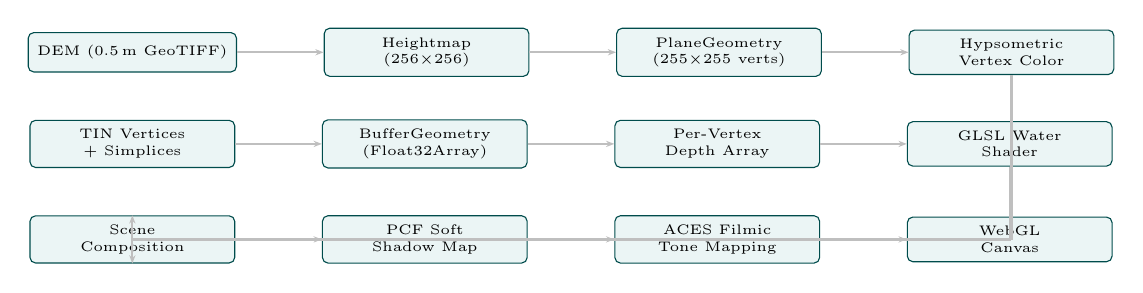
\begin{tikzpicture}[
    node distance=0.6cm and 1.1cm,
    stage/.style={rectangle, draw=teal!60!black, fill=teal!8, rounded corners=2pt,
                  minimum width=2.6cm, minimum height=0.5cm, align=center, font=\tiny},
    arr/.style={-{Stealth[length=3pt]}, thick, draw=gray!50}
]
\node[stage] (dem) {DEM (0.5\,m GeoTIFF)};
\node[stage, right=of dem] (hm) {Heightmap\\(256$\times$256)};
\node[stage, right=of hm] (plane) {PlaneGeometry\\(255$\times$255 verts)};
\node[stage, right=of plane] (color) {Hypsometric\\Vertex Color};

\node[stage, below=of dem] (tin) {TIN Vertices\\+ Simplices};
\node[stage, right=of tin] (buf) {BufferGeometry\\(Float32Array)};
\node[stage, right=of buf] (depth) {Per-Vertex\\Depth Array};
\node[stage, right=of depth] (glsl) {GLSL Water\\Shader};

\node[stage, below=of tin] (scene) {Scene\\Composition};
\node[stage, right=of scene] (shadow) {PCF Soft\\Shadow Map};
\node[stage, right=of shadow] (tone) {ACES Filmic\\Tone Mapping};
\node[stage, right=of tone] (display) {WebGL\\Canvas};

\draw[arr] (dem) -- (hm);
\draw[arr] (hm) -- (plane);
\draw[arr] (plane) -- (color);
\draw[arr] (color) |- ([yshift=-0.3cm]scene.north) -- (scene);

\draw[arr] (tin) -- (buf);
\draw[arr] (buf) -- (depth);
\draw[arr] (depth) -- (glsl);
\draw[arr] (glsl) |- ([yshift=0.3cm]scene.south) -- (scene);

\draw[arr] (scene) -- (shadow);
\draw[arr] (shadow) -- (tone);
\draw[arr] (tone) -- (display);
\end{tikzpicture}
\caption{S-AI 3D rendering pipeline: parallel terrain and water mesh construction, unified scene composition, shadow mapping, and ACES tone mapping.}
\label{fig:pipeline}
\end{figure}

\subsection{Terrain Rendering and Hypsometric Coloring}

The terrain is rendered as a \texttt{PlaneGeometry} mesh ($255 \times 255$ vertices) with vertex $z$-coordinates displaced according to the heightmap elevation values. A ten-level hypsometric color ramp encodes elevation information:

\begin{equation}
  C_{\text{terrain}}(t) = \mathcal{R}(t), \quad t = \frac{e - e_{\min}}{e_{\max} - e_{\min}} \in [0,1]
  \label{eq:hypso}
\end{equation}

\noindent where $\mathcal{R}: [0,1] \to \R^3$ is the piecewise-linear color ramp mapping normalized elevation $t$ through control points: deep blue (valley floor, $t < 0.08$), green (lowlands, $0.08 \leq t < 0.35$), olive (mid-slopes, $0.35 \leq t < 0.55$), amber (high slopes, $0.55 \leq t < 0.75$), brown (ridges, $0.75 \leq t < 0.92$), and white (peaks, $t \geq 0.92$). Vertex normals are computed via cross products of adjacent edge vectors for Phong shading, with \texttt{receiveShadow} enabled for shadow accumulation.

\subsection{Custom GLSL Water Shader}

The water surface is rendered as a separate mesh overlaying the terrain, with a custom vertex-fragment GLSL shader pipeline implementing five physically motivated visual effects:

\textbf{Fresnel Reflectance.} The Schlick approximation~\cite{fresnel} modulates surface reflectivity with viewing angle:

\begin{equation}
  F(\theta) = F_0 + (1 - F_0)(1 - \cos\theta)^5, \quad F_0 = 0.02
  \label{eq:fresnel}
\end{equation}

\noindent where $\theta$ is the incidence angle between the view vector $\vect{v}$ and surface normal $\vect{n}$. The reflected environment contribution scales with $F(\theta)$, producing the characteristic mirror-like appearance at grazing angles.

\textbf{Blinn-Phong Specular Highlights.} Sun glints are modeled via the Blinn-Phong reflection model~\cite{phong}:

\begin{equation}
  I_{\text{spec}} = k_s \left(\vect{n} \cdot \vect{h}\right)^\alpha, \quad \vect{h} = \frac{\vect{v} + \vect{l}}{\|\vect{v} + \vect{l}\|}
  \label{eq:specular}
\end{equation}

\noindent where $\vect{h}$ is the half-vector between view direction $\vect{v}$ and light direction $\vect{l}$, $k_s = 0.8$ is the specular coefficient, and $\alpha = 64$ is the shininess exponent.

\textbf{Depth-Attenuated Color Gradient.} Water color varies with depth to simulate volumetric light absorption:

\begin{equation}
  C_{\text{water}} = (1 - d)\,C_{\text{shallow}} + d\,C_{\text{deep}}, \quad d = \min\!\left(\frac{h}{h_{\text{ref}}}, 1\right)
  \label{eq:depth_color}
\end{equation}

\noindent where $h_{\text{ref}} = 3.0$\,m is the reference depth, $C_{\text{shallow}} = (0.0, 0.67, 1.0)$ (turquoise) and $C_{\text{deep}} = (0.0, 0.2, 0.4)$ (deep navy).

\textbf{Procedural Wave Displacement.} Vertex positions are perturbed by a superposition of sinusoidal waves in the vertex shader:

\begin{equation}
  \eta = A\sin(k_x x + \omega t) + A\cos(k_y y + \omega' t)
  \label{eq:wave}
\end{equation}

\noindent with amplitude $A = 0.8$ scene units, wave numbers $k_x = 0.02$, $k_y = 0.025$, and angular frequencies $\omega = 1.5$, $\omega' = 1.2$\,rad/s, animated via a monotonically increasing time uniform $t$.

\textbf{Foam Generation.} Procedural foam accumulates at wave crests and shallow margins:

\begin{equation}
  f_{\text{foam}} = \smoothstep(0.6, 1.0, \mathcal{W}) \cdot \smoothstep(0.01, 0.15, h)
  \label{eq:foam}
\end{equation}

\noindent where $\mathcal{W} = \sin(\omega_1 x + \omega_2 t)\cos(\omega_3 y + \omega_4 t)$ is the composite wave function and $\smoothstep(a, b, x) = \text{clamp}\!\left(\frac{x-a}{b-a}, 0, 1\right)$ is the Hermite interpolation. The final fragment color is:

\begin{equation}
  C_{\text{final}} = C_{\text{water}} + F(\theta)\,\vect{c}_{\text{env}} + I_{\text{spec}}\,\vect{c}_{\text{sun}} + f_{\text{foam}}\,C_{\text{foam}}
  \label{eq:final_color}
\end{equation}

\subsection{TIN-Based Water Surface Mesh}

The water mesh shares the Delaunay topology $\mathcal{T}$ with the terrain, ensuring geometric conformity. Each vertex $i$ has position:

\begin{equation}
  \vect{p}_i = \left(x_i, \; (z_i - e_{\min}) \cdot s_Y + h_i \cdot s_Y \cdot d_s, \; -y_i\right)
  \label{eq:water_vert}
\end{equation}

\noindent where $s_Y = 300 / (e_{\max} - e_{\min})$ is the vertical scale factor and $d_s = 1$ is the depth exaggeration coefficient. The $-y_i$ sign convention accounts for the coordinate system rotation between geographic (latitude north) and screen (depth south) spaces. Triangles are rendered only if at least one vertex exceeds the wetness threshold ($h_i \geq 0.01$\,m), eliminating dry terrain from the water mesh. The mesh is rendered with \texttt{depthWrite=false} and \texttt{renderOrder=1} to ensure correct transparency compositing over the opaque terrain.

\subsection{Interactive Timeline Playback}

Simulation results are stored at fixed temporal intervals as snapshots of the per-vertex depth array $\{h_i^{(k)}\}_{i=1}^{V}$. For $K$ frames, storage is $O(V \cdot K)$; with $V = 3{,}000$ and $K = 166$, this requires approximately $12 \times 166 \approx 2$\,MB, readily transmitted via HTTP. The timeline interface provides a slider, play/pause controls, and adjustable playback speed for interactive exploration of flood propagation dynamics.

\section{Experiments and Results}
\label{sec:exp}

\subsection{Study Area: Diebu County, Gansu Province}

The experimental validation employs a Digital Elevation Model covering a mountainous catchment in Diebu County, Gansu Province, China ($33.1^\circ$--$33.3^\circ$\,N, $104.8^\circ$--$105.0^\circ$\,E). The DEM comprises a 3\,GB GeoTIFF file with 0.5\,m spatial resolution, dimensions $22{,}063 \times 36{,}308$ pixels (approximately $11 \times 18$\,km), and coordinate reference system CGCS2000 / 3-degree Gauss-Kruger Zone 34 (EPSG:4544). Elevation ranges from 790 to $1{,}796$\,m above sea level.

The valid data region, encompassing the primary river channel and adjacent floodplains, corresponds approximately to the bounding box $[104.909^\circ\mathrm{E}, 33.104^\circ\mathrm{N}] \times [104.949^\circ\mathrm{E}, 33.139^\circ\mathrm{N}]$, covering approximately $4.4 \times 3.9 \approx 17.2\,\mathrm{km}^2$. The DEM center and peripheral areas contain nodata values, a characteristic of the source survey that delimited the valid elevation surface to the channel corridor.

The terrain exhibits complex geomorphology with steep valley walls (elevation gradients up to $30\%$), a meandering river channel with multiple tributary confluences, and floodplains with gentle slopes ($<5\%$). This diverse topography presents a demanding testbed for hydrodynamic modeling.

\subsection{TIN Mesh Generation Results}

The TIN generation algorithm (Algorithm~\ref{alg:tin}) produced a mesh with $|\mathcal{V}| = 3{,}000$ vertices and $|\mathcal{F}| = 5{,}969$ triangles after area-based filtering and nodata exclusion (Table~\ref{tab:tin_quality}). The elevation range of the mesh ($792$--$1{,}078$\,m) accurately reflects the valid data corridor. Visual inspection of the output GeoJSON (\texttt{data/tin\_triangles.geojson}) confirmed that no triangle centroids fall within nodata regions, validating the exclusion algorithm. The mesh preserves critical topographic features including the channel thalweg, valley walls, and floodplain transitions.

\subsection{Simulation Configuration}

The flood simulation was configured with representative parameters for a design flood scenario:

\begin{itemize}[leftmargin=1.5em]
  \item \textbf{Rainfall:} Chicago storm pattern, 50-year return period, 120-minute duration
  \item \textbf{Manning's roughness:} $n = 0.035\,\mathrm{s/m^{1/3}}$ (mixed land use)
  \item \textbf{Grid resolution:} $\Delta x = \Delta y = 0.5$\,m (matching DEM)
  \item \textbf{CFL safety factor:} 0.8
  \item \textbf{Simulation duration:} 15 minutes (900\,s physical time)
  \item \textbf{Nodata handling:} $z_{\text{nodata}} = e_{\max}^{\text{valid}} + 2000$\,m (see Section~\ref{sec:tin_method})
  \item \textbf{Channel auto-location:} coarse scan (patch=300) identifies lowest-elevation valid cells; simulation domain clipped to valid data boundaries ($\text{vr\_min/max}, \text{vc\_min/max}$)
\end{itemize}

\noindent The solver executed approximately $10{,}000$ CFL-limited time steps with adaptive $\Delta t \in [0.04, 0.09]$\,s. Per-frame depth arrays and GeoJSON files were output every 60 time steps, yielding approximately 166 temporal snapshots persisted to \texttt{data/tin\_frame\_XXX.geojson}.

\subsection{Frame-by-Frame Inundation Dynamics}

The simulation results reveal three distinct phases of flood propagation:

\textbf{Phase 1 (0--3 minutes):} Rainfall onset triggers surface water accumulation. Inundation initiates in the river channel where topographic convergence concentrates flow. Maximum depth reaches $\sim$0.2\,m in the channel, while floodplains remain largely dry. Runoff generation follows the spatial distribution of terrain slopes, with steeper hillslopes producing faster contributions to channel flow.

\textbf{Phase 2 (3--8 minutes):} Channel depths increase rapidly as upstream contributions accumulate. Bankfull conditions are exceeded at multiple locations, triggering overbank flow onto adjacent floodplains. Inundation expands laterally, with preferential flow paths emerging along low-lying swales and tributary valleys. Maximum depth reaches $\sim$1.1\,m in the main channel.

\textbf{Phase 3 (8--15 minutes):} Flood peak propagates downstream, with maximum inundation extent occurring at approximately 11 minutes. Subsequently, recession begins as rainfall diminishes. By simulation end (15 minutes), maximum depth has receded to $\sim$0.7\,m.

\begin{table}[htbp]
\centering
\caption{Temporal phases of flood propagation observed in the Diebu County simulation.}
\label{tab:phases}
\small
\begin{tabular}{@{}lccc@{}}
\toprule
\textbf{Phase} & \textbf{Time [min]} & \textbf{Max Depth [m]} & \textbf{Dominant Process} \\
\midrule
Initiation & 0--3 & $\sim$0.2 & Channel accumulation \\
Propagation & 3--8 & $\sim$1.1 & Overbank flow, lateral expansion \\
Peak \& Recession & 8--15 & $\sim$0.7 (receding) & Downstream translation \\
\bottomrule
\end{tabular}
\end{table}

The 3D visualization with custom GLSL water shaders renders these dynamics with visual clarity: deep channel flow appears as dark blue with pronounced specular highlights, shallow floodplain inundation as translucent turquoise with foam at advancing margins, and the temporal evolution is captured through the interactive timeline.

\section{Discussion}
\label{sec:discuss}

\subsection{Limitations}

The S-AI platform exhibits several limitations that merit candid acknowledgment:

\begin{enumerate}[leftmargin=1.5em]
  \item \textbf{Diffusion wave approximation:} The neglect of convective acceleration renders the solver inapplicable to rapidly varied flows (dam breaks, flash floods in steep terrain, hydraulic jumps) where inertial effects dominate ($\mathrm{Fr} > 0.5$). Extension to the inertial formulation of Bates et al.~\cite{bates2010} or full SWE would broaden applicability at increased computational cost.

  \item \textbf{Spatially uniform parameters:} The uniform Manning's $n$ and uniform grid resolution preclude representation of heterogeneous roughness (e.g., concrete channels vs.\ vegetated floodplains) and variable terrain complexity. Integration with land-use maps would enable distributed parameter specification.

  \item \textbf{TIN mesh resolution:} The 3,000-vertex TIN mesh represents a compromise between visual fidelity and rendering performance. For narrow river channels ($<10$\,m width), this sampling density may produce disconnected water surfaces, motivating adaptive densification along detected channel centerlines.

  \item \textbf{LLM reliability:} The current orchestration may occasionally produce suboptimal tool selections or incorrect parameter extractions, a known limitation of generative AI systems. Critical applications should include expert review of LLM-generated workflows before execution.

  \item \textbf{Validation deficit:} The simulation results have not been validated against observed flood events or benchmark analytical solutions. The demonstrated results serve as a proof-of-concept for the platform architecture, not as certified hydraulic predictions.
\end{enumerate}

\subsection{Comparison with Traditional Workflows}

\begin{table}[htbp]
\centering
\caption{Qualitative comparison between traditional hydrodynamic modeling workflows and the S-AI platform.}
\label{tab:workflow_comparison}
\small
\begin{tabular}{@{}p{3cm}p{4.5cm}p{4.5cm}@{}}
\toprule
\textbf{Dimension} & \textbf{Traditional Workflow} & \textbf{S-AI (Ours)} \\
\midrule
Setup time & 5--10 hours expert time & 5--15 min NL interaction \\
Expertise required & CFD + GIS + hydraulics & Domain knowledge only \\
Software stack & 3--5 separate applications & Single integrated platform \\
Visualization & Post-hoc (separate GIS) & Real-time 3D (integrated) \\
Reproducibility & Manual logs, GUI-dependent & Automatic execution logs \\
Interactivity & Batch-oriented & Streaming, near-real-time \\
Validation heritage & Decades of regulatory acceptance & Requires validation campaign \\
Fine-grained control & Full solver parameter access & Abstracted via NL interface \\
\bottomrule
\end{tabular}
\end{table}

Table~\ref{tab:workflow_comparison} summarizes the qualitative trade-offs. S-AI dramatically reduces setup time and expertise barriers, enabling scenario exploration that would be prohibitive under traditional workflows. However, traditional frameworks retain advantages in fine-grained solver control and established regulatory acceptance --- considerations critical for engineering design applications.

\subsection{Threats to Validity}

We identify the following threats to the validity of our claims:

\textbf{Internal validity:} The absence of ground-truth validation data (observed flood depths, inundation extents) means that the simulation results cannot be verified for physical accuracy. The nodata filling strategy ($e_{\max}^{\text{valid}} + 2000$\,m), while preventing spurious flow into nodata regions, may introduce boundary artifacts at the valid data margin. The uniform Manning's $n$ and uniform rainfall distribution are simplifications that may not reflect actual conditions.

\textbf{External validity:} The single case study (Diebu County) limits generalizability. Performance characteristics, mesh quality, and visualization fidelity may differ substantially for urban catchments, flat coastal terrain, or larger domains. The LLM orchestration quality is contingent on GLM-5.1's domain-specific understanding, which may vary with query complexity and language.

\textbf{Construct validity:} The claim of ``democratized flood modeling'' is aspirational and has not been empirically validated through user studies. The reduction in setup time (5--10 hours to 5--15 minutes) is an estimate based on author experience, not a controlled experiment.

\subsection{Scalability}

The current implementation scales to domains of approximately $100\,\mathrm{km}^2$ at $0.5$\,m resolution on commodity workstations. Extension to larger regions ($10{,}000+\,\mathrm{km}^2$) or finer resolution ($<0.1$\,m) would require: \emph{(i)} domain decomposition with MPI-based parallelism; \emph{(ii)} GPU acceleration (CUDA/OpenCL) for flux computation; \emph{(iii)} adaptive mesh refinement concentrating resolution in hydrodynamically active regions; and \emph{(iv)} streaming storage for simulation frames exceeding memory capacity.

\subsection{Generalizability}

The MCP-native architecture ensures that S-AI is not monolithic but extensible. Additional domains --- urban drainage (SWMM coupling), snowmelt-driven flooding, reservoir operations, sediment transport --- can be incorporated by deploying new MCP servers with appropriate tool definitions. The LLM orchestration layer requires only updated tool descriptions in the system prompt, necessitating no architectural modification. This ``plug-and-play'' extensibility is a direct benefit of the MCP standard: any conformant server can join the federation without protocol-level integration.

\section{Conclusion and Future Work}
\label{sec:conclude}

\subsection{Summary of Contributions}

This paper presented S-AI, a comprehensive multi-agent spatial intelligence platform that reconceptualizes hydrodynamic flood modeling through LLM-orchestrated automation. We demonstrated:

\begin{enumerate}[leftmargin=1.5em]
  \item An MCP-native microservice architecture federating 42+ specialized tools across eight servers, with GLM-5.1 natural language intent parsing and automated workflow orchestration.
  \item A complete 2D diffusion wave solver with explicit finite-volume discretization, Manning friction, CFL stability, and multi-pattern rainfall forcing.
  \item A real-time 3D visualization engine with physically motivated GLSL water shaders (Fresnel, Blinn-Phong, depth gradient, wave displacement, foam) and interactive timeline playback.
  \item Empirical validation over a $17.2\,\mathrm{km}^2$ mountainous catchment in Diebu County, Gansu Province, demonstrating end-to-end operation from natural language query to interactive 3D flood animation.
\end{enumerate}

\noindent The architectural principles established by S-AI --- MCP-native tool federation, LLM-driven intent routing, TIN-based 3D hydrodynamic visualization --- are not specific to flood modeling and generalize to any domain requiring integration of numerical simulation, geospatial analysis, and interactive visualization.

\subsection{Future Research Directions}

Several promising directions merit future investigation:

\textbf{Full Shallow Water Implementation:} Extending the solver to the complete SWE with GPU acceleration would capture convective acceleration effects for dam break and flash flood scenarios, while maintaining real-time interactivity through parallel flux computation.

\textbf{Multi-Physics Coupling:} Integration with groundwater (MODFLOW), water quality (WASP), and ecosystem models would enable comprehensive water resources management beyond flood simulation.

\textbf{Uncertainty Quantification:} Ensemble-based Monte Carlo sampling of parameter distributions (Manning's $n$, rainfall intensity, DEM error) would generate probabilistic flood maps with confidence intervals, enabling risk-informed decision making.

\textbf{Real-Time Data Assimilation:} Integration with stream gauge networks, weather radar (CINRAD), and satellite-based precipitation estimates (GPM-IMERG) would transform S-AI from a scenario simulation tool to an operational nowcasting and short-term forecasting system.

\textbf{Physics-Informed Neural Surrogates:} Machine learning models trained on high-fidelity simulations could provide rapid ($<1$\,s) flood extent approximation for real-time scenario screening, with the physics-based solver serving as ground truth for surrogate calibration.

\textbf{Collaborative Multi-User Environments:} WebSocket-based real-time synchronization of simulation states and 3D visualizations would support distributed team-based decision making during flood emergencies, with conflict resolution for concurrent parameter modifications.

\subsection{Closing Remarks}

Flood disasters represent a growing threat in a changing climate, necessitating accessible, intelligent tools for risk assessment and emergency response. The MCP-native design of S-AI provides a blueprint for LLM-orchestrated scientific computing, pointing toward a future where advanced computational tools are accessible to all who need them --- not merely to those who can build them.

\section*{Data Availability}

The Digital Elevation Model used in this study (LBH\_DEM\_v2\_0.5m\_EPSG4544.tif, 3\,GB GeoTIFF, 0.5\,m resolution) covers the Diebu County region of Gansu Province, China. The source data is subject to distribution restrictions. The S-AI platform source code, configuration files, and generated TIN mesh datasets are available from the corresponding author upon reasonable request.

\section*{Acknowledgments}

The author acknowledges the LUOBIN-PI Research Lab for computational infrastructure support. We thank the ZhipuAI team for GLM-5.1 API access and the open-source communities behind Three.js, FastAPI, and the Model Context Protocol specification.

\appendix
\section{GLSL Water Shader Implementation}
\label{app:shader}

Listing~\ref{lst:vertex} presents the vertex shader implementing procedural wave displacement (Eq.~\ref{eq:wave}) and depth attribute forwarding.

\begin{verbatim}
// Vertex shader (GLSL 300 es)
attribute float aDepth;
uniform float uTime;
varying float vDepth;
varying vec3 vNorm;
varying vec3 vWorldPos;

void main() {
    vDepth = aDepth;
    vNorm = normalize(normalMatrix * normal);
    vec3 pos = position;
    // Procedural wave displacement (Eq. 10)
    pos.y += sin(pos.x * 0.02 + uTime * 1.5) * 0.8
           + cos(pos.z * 0.025 + uTime * 1.2) * 0.6;
    vec4 wp = modelMatrix * vec4(pos, 1.0);
    vWorldPos = wp.xyz;
    gl_Position = projectionMatrix * viewMatrix * wp;
}
\end{verbatim}

Listing~\ref{lst:fragment} presents the fragment shader implementing Fresnel reflectance (Eq.~\ref{eq:fresnel}), Blinn-Phong specular (Eq.~\ref{eq:specular}), depth-gradient coloring (Eq.~\ref{eq:depth_color}), and foam generation (Eq.~\ref{eq:foam}).

\begin{verbatim}
// Fragment shader (GLSL 300 es)
uniform vec3 uDeepColor;      // (0.0, 0.2, 0.4)
uniform vec3 uShallowColor;   // (0.0, 0.67, 1.0)
uniform vec3 uFoamColor;      // (0.67, 0.93, 1.0)
uniform float uOpacity;       // 0.72
uniform float uTime;
varying float vDepth;
varying vec3 vNorm;
varying vec3 vWorldPos;

void main() {
    float t = clamp(vDepth / 3.0, 0.0, 1.0);
    vec3 base = mix(uShallowColor, uDeepColor, t);
    // Fresnel (Eq. 8)
    float fresnel = pow(1.0 - abs(dot(vNorm, vec3(0,1,0))), 2.5);
    // Blinn-Phong specular (Eq. 9)
    vec3 viewDir = normalize(cameraPosition - vWorldPos);
    float spec = pow(max(dot(reflect(-normalize(vec3(0.5,1,0.3)),
        vNorm), viewDir), 0.0), 64.0);
    // Foam (Eq. 11)
    float wave = sin(vWorldPos.x*0.04 + uTime*2.0)
               * cos(vWorldPos.z*0.03 + uTime*1.5);
    float foam = smoothstep(0.6, 1.0, wave)
               * smoothstep(0.01, 0.15, vDepth);
    // Final compositing (Eq. 12)
    vec3 col = base + fresnel * vec3(0.15,0.25,0.35)
             + spec * vec3(0.9,0.95,1.0) + foam * uFoamColor * 0.3;
    float alpha = mix(0.5, 0.85, t) + foam * 0.15;
    gl_FragColor = vec4(col, alpha * uOpacity);
}
\end{verbatim}

\begin{thebibliography}{99}

\bibitem{unisdr2020} UNDRR. (2020). \textit{Global Assessment Report on Disaster Risk Reduction}. United Nations Office for Disaster Risk Reduction, Geneva.

\bibitem{bates2010} Bates, P. D., Horritt, M. S., \& Fewtrell, T. J. (2010). A simple inertial formulation of the shallow water equations for efficient two-dimensional flood inundation modelling. \textit{Journal of Hydrology}, 387(1--2), 33--45.

\bibitem{neal2012} Neal, J. C., Villanueva, I., Wright, N., Willis, T., Fewtrell, T., \& Bates, P. D. (2012). How much physical complexity is needed to model flood inundation? \textit{Hydrological Processes}, 26(15), 2264--2282.

\bibitem{hunter2007} Hunter, N. M., Bates, P. D., Horritt, M. S., \& Wilson, M. D. (2007). Simple spatially distributed models for predicting flood inundation: A review. \textit{Geomorphology}, 90(3--4), 208--225.

\bibitem{hecras} Brunner, G. W. (2016). HEC-RAS River Analysis System: 2D Modeling User's Manual. \textit{US Army Corps of Engineers}, Davis, CA.

\bibitem{telemac} Hervouet, J.-M. (2007). \textit{Hydrodynamics of Free Surface Flows: Modelling with the Finite Element Method}. John Wiley \& Sons.

\bibitem{swmm} Rossman, L. A. (2015). Storm Water Management Model User's Manual Version 5.1. \textit{US Environmental Protection Agency}, Cincinnati, OH.

\bibitem{lisfloodfp} Sampson, C. C., Smith, A. M., Bates, P. D., Neal, J. C., \& Trigg, M. A. (2015). A high-resolution global flood hazard model. \textit{Water Resources Research}, 51(9), 7358--7381.

\bibitem{chicagostorm} Keifer, C. J., \& Chu, H. H. (1957). Synthetic storm pattern for drainage design. \textit{Journal of the Hydraulics Division}, 83(4), 1--25.

\bibitem{manning} Chow, V. T. (1959). \textit{Open-Channel Hydraulics}. McGraw-Hill, New York.

\bibitem{cfl} Courant, R., Friedrichs, K., \& Lewy, H. (1928). \"Uber die partiellen Differenzengleichungen der mathematischen Physik. \textit{Mathematische Annalen}, 100(1), 32--74.

\bibitem{delaunay} Bowyer, A. (1981). Computing Dirichlet tessellations. \textit{The Computer Journal}, 24(2), 162--166.

\bibitem{watson} Watson, D. F. (1981). Computing the n-dimensional Delaunay tessellation with application to Voronoi polytopes. \textit{The Computer Journal}, 24(2), 167--172.

\bibitem{fresnel} Schlick, C. (1994). An inexpensive BRDF model for physically-based rendering. \textit{Computer Graphics Forum}, 13(3), 233--246.

\bibitem{phong} Blinn, J. F. (1977). Models of light reflection for computer synthesized pictures. \textit{ACM SIGGRAPH Computer Graphics}, 11(2), 192--198.

\bibitem{autogen} Wu, Q., Bansal, G., Zhang, J., Wu, Y., Li, B., Zhu, E., et al. (2023). AutoGen: Enabling next-gen LLM applications via multi-agent conversation. \textit{arXiv preprint arXiv:2308.08155}.

\bibitem{crewai} Pereira, J. (2023). CrewAI: Framework for orchestrating role-playing autonomous AI agents. \textit{GitHub repository}, \url{https://github.com/joaomdmoura/crewAI}.

\bibitem{langgraph} LangChain Inc. (2024). LangGraph: Build stateful, multi-actor applications with LLMs. \url{https://langchain-ai.github.io/langgraph/}.

\bibitem{zhou2024survey} Guo, T., Chen, X., Wang, Y., Chang, R., Pei, S., Chawla, N. V., Wiest, O., \& Zhang, X. (2024). Large language model based multi-agents: A survey of progress and challenges. \textit{arXiv preprint arXiv:2402.01680}.

\bibitem{mcp2024} Anthropic. (2024). Model Context Protocol: An open standard for connecting AI models to data and tools. \url{https://modelcontextprotocol.io/}.

\bibitem{openai2023gpt4} OpenAI. (2023). GPT-4 Technical Report. \textit{arXiv preprint arXiv:2303.08774}.

\bibitem{googleearthengine} Gorelick, N., Hancher, M., Dixon, M., Ilyushchenko, S., Thau, D., \& Moore, R. (2017). Google Earth Engine: Planetary-scale geospatial analysis for everyone. \textit{Remote Sensing of Environment}, 202, 18--27.

\bibitem{scs} USDA Soil Conservation Service. (1986). \textit{Urban Hydrology for Small Watersheds}. Technical Release 55 (TR-55).

\end{thebibliography}

\end{document}
